\documentclass{scrartcl}

\usepackage{amsmath}	  % required for math in general
\usepackage{amsthm}     % environments for theorems, qed's etc
                        % (loaded after amsmath)
\usepackage{amssymb}	  % doublestroke symbols, other mathematical symbols
%\usepackage{dsfont}     % required for double-stroke 1 as characteristic function
\usepackage{array}	    % control of matrices and tables
\usepackage{graphicx}   % images

\usepackage{enumitem}   % more fine-grained control over enumerations
\setdescription{leftmargin=\parindent,labelindent=\parindent}

\usepackage{listings} % code listings
\lstset{basicstyle=\ttfamily\scriptsize}

% \input{diagrams.sty} (no category theory this time)

\usepackage{helvet}   % use (much fresher looking) helvetica for everything
\renewcommand{\familydefault}{\sfdefault}

\usepackage[weather]{ifsym}      % \Lightning symbol
% \usepackage{mathabx}             % \Asterisk causes some conflicts

% forcing the fucking floats to stop fucking floating like a fucking piece of
% shit in an ocean of fucking shit
\renewcommand{\topfraction}{.85}
\renewcommand{\bottomfraction}{.7}
\renewcommand{\textfraction}{.15}
\renewcommand{\floatpagefraction}{.66}
\renewcommand{\dbltopfraction}{.66}

% making all references into hyperlinks
\usepackage[dvipsnames]{xcolor}
\usepackage{hyperref}

\hypersetup{colorlinks=true,linkcolor=MidnightBlue,pdfborderstyle={/W 0}}

%\usepackage{anyfontsize}
\usepackage{datetime}

% forall
\let\oldforall\forall
\renewcommand{\forall}{\oldforall\,}

% parentheses
\newcommand{\rPar}[1]{\left(#1\right)} % round parens
\newcommand{\sPar}[1]{\left[#1\right]} % square parens
\newcommand{\cPar}[1]{\left\{#1\right\}} % curved parens 
\newcommand{\aPar}[1]{\left\langle #1 \right\rangle} % angle brackets

% floor and ceiling
\newcommand{\floor}[1]{{\left\lfloor#1\right\rfloor}} % curved parens 
\newcommand{\ceil}[1]{{\left\lceil#1\right\rceil}} % curved parens 

% norms
\newcommand{\abs}[1]{\left\lvert #1\right\rvert}
\newcommand{\norm}[1]{\left\lVert #1\right\rVert}
\newcommand{\scalar}[2]{\left\langle#1,#2\right\rangle}
\newcommand{\cross}{\times}
\DeclareMathOperator{\diam}{diam}
\DeclareMathOperator{\B}{B}

% intervals
\newcommand{\openOpenInterval}[2]{{\left(#1,#2\right)}}
\newcommand{\openClosedInterval}[2]{{\left(#1,#2\right]}}
\newcommand{\closedOpenInterval}[2]{{\left[#1,#2\right)}}
\newcommand{\closedClosedInterval}[2]{{\left[#1,#2\right]}}

% restriction of functions
\newcommand{\restrict}[2]{{\left.#1\right\vert_{#2}}}

% numbers
\newcommand{\Natural}{\mathbb{N}}
\newcommand{\Integer}{\mathbb{Z}}
\newcommand{\Real}{\mathbb{R}}
\newcommand{\Rational}{\mathbb{Q}}
\newcommand{\PositiveReal}{\Real_{>0}}
\newcommand{\NonnegativeReal}{\Real_{\geq0}}
\newcommand{\Complex}{\mathbb{C}}
\renewcommand{\i}{i}
\newcommand{\Quaternion}{\mathbb{H}}
\newcommand{\Boolean}{\mathbb{B}}

% function spaces
\newcommand{\SemiLebesgue}{\mathscr{L}}
\newcommand{\Continuous}{C}
\newcommand{\Lebesgue}{L}
\newcommand{\Sobolev}{H}
\newcommand{\Hilbert}{\mathscr{H}}
\newcommand{\Schwarz}{\mathscr{S}}

% set
\newcommand{\setPredicate}[2]{{\left\{#1\,\left\vert\, #2\right.\right\}}}
\newcommand{\set}[1]{{\left\{#1\right\}}}
\newcommand{\cardinality}[1]{\left\lvert #1 \right\rvert}
\newcommand{\powerset}[1]{\mathfrak{P}\left(#1\right)}
\DeclareMathOperator*{\intersection}{\bigcap}
\DeclareMathOperator*{\union}{\bigcup}
\newcommand{\disjointUnion}{\biguplus}
\renewcommand{\complement}[1]{#1^c}
% \newcommand{\setminus}{\backslash}
\newcommand{\injective}{\hookrightarrow}
\newcommand{\surjective}{\twoheadrightarrow}
%\DeclareMathOperator{\ker}{ker} % already exists... im does not?
\DeclareMathOperator{\im}{im}

% topological operators
\DeclareMathOperator{\Cl}{Cl}
\newcommand{\Closure}[2]{\Cl_{#1}\left(#2\right)}
\DeclareMathOperator{\const}{const}

% span and conv
\DeclareMathOperator*{\conv}{conv}
\DeclareMathOperator*{\linhull}{span}

% matrices
\newcommand{\mat}[2]{\left[\begin{array}{#1}#2\end{array}\right]}
\DeclareMathOperator*{\diag}{diag}

% landau symbols
\newcommand{\LandauO}[1]{\mathcal{O}\left(#1\right)}

% derivatives
\newcommand{\dd}[2]{\frac{\partial #1}{\partial #2}}
\newcommand{\differential}[1]{\boldsymbol{D}_{#1}}

% integrals
\renewcommand{\d}{\quad\mathrm{d}}

% characteristic functions, expected values, variances, covariances
% stochastic stuff
\newcommand{\one}[1]{\mathds{1}_{#1}}
\newcommand{\weakconv}[1]{\overset{#1}{\Longrightarrow}}
\newcommand{\wlim}{\mathop{\mathrm{wlim}}}
\newcommand{\vlim}{\mathop{\mathrm{vlim}}}

% lim inf lim sup
% \DeclareMathOperator{\liminf}{lim inf}
% \DeclareMathOperator{\limsup}{lim sup}

% qed etc.
\renewcommand{\qedsymbol}{$\blacksquare$}
\newcommand{\result}{\hfill $\Diamond$}

% lattices
\newcommand{\meet}{\wedge}
\newcommand{\join}{\vee}
\newcommand{\negate}{\neg}

% listings: Scala
\lstdefinelanguage{scala}{
  morekeywords={abstract,case,catch,class,def,%
    do,else,extends,false,final,finally,%
    for,if,implicit,import,match,mixin,%
    new,null,object,override,package,%
    private,protected,requires,return,sealed,%
    super,this,throw,trait,true,try,%
    type,val,var,while,with,yield},
  otherkeywords={=>,<-,<\%,<:,>:,\#,@},
  sensitive=true,
  morecomment=[l]{//},
  morecomment=[n]{/*}{*/},
  morestring=[b]",
  morestring=[b]',
  morestring=[b]"""
}
\lstset{showstringspaces=false}

% making references look a little nices
\let\oldRef\ref
\renewcommand{\ref}[1]{(\oldRef{#1})}

% weird stuff for computer science
\DeclareMathOperator{\arity}{ar}

% cat, category theory
% Bunch of categories
\DeclareMathOperator{\Id}{Id}
\DeclareMathOperator{\Top}{Top}
\DeclareMathOperator{\hTop}{h-Top}
\DeclareMathOperator{\Sets}{Sets}
\DeclareMathOperator{\Rel}{Rel}
\DeclareMathOperator{\FinSets}{FinSets}
\DeclareMathOperator{\Grp}{Grp}
\DeclareMathOperator{\Cat}{Cat}
\DeclareMathOperator{\Grpd}{Grpd}
\newcommand{\cat}[1]{\mathcal{#1}}
\newcommand{\Obj}{\mathrm{Obj}}
\newcommand{\Hom}{\mathrm{Hom}}
\newcommand{\op}{\mathrm{op}}
\newcommand{\nat}{\xrightarrow{\bullet}}
\newcommand{\iso}{\cong}
\newcommand{\dom}{\mathrm{dom}}
\newcommand{\cod}{\mathrm{cod}}
\DeclareMathOperator{\coeq}{Coeq}
\newcommand{\fst}{\mathrm{fst}}
\newcommand{\snd}{\mathrm{snd}}
\DeclareMathOperator{\Aut}{Aut}
\DeclareMathOperator{\End}{End}

% functors frequently used in various contexts
\DeclareMathOperator{\Free}{Free}
\DeclareMathOperator{\Forget}{Forget}

% empty set that is round
\let\emptyset\varnothing

% generated groups
\newcommand{\gen}[1]{\left\langle#1\right\rangle}
\newcommand{\normalSub}{\triangleleft}
\newcommand{\Asterisk}{\mathop{\scalebox{1.5}{\raisebox{-0.2ex}{$\ast$}}}}
\newcommand{\Sym}{\mathrm{Sym}}

% argmax argmin argsup etc.
\DeclareMathOperator{\argsup}{argsup}

% number theoretic operators
\DeclareMathOperator{\lcm}{lcm}

% get rid of the ugly-looking "epsilon"
\renewcommand{\epsilon}{\varepsilon}

% get rid of the empty-looking "angle"
\renewcommand{\angle}{\measuredangle}

\newcommand{\exercise}[2]{\vspace{1em}\noindent{\bf Exercise #1 (#2)}}
\renewcommand{\proof}{\vspace{0.8em}\noindent{\bf Proof: }}

\begin{document}
\noindent{\footnotesize Computer Graphics 2014/15, Exercise 4} 
\hfill 
{\footnotesize 14.01.2015}
\newline
{\footnotesize \input{../../NAMES.txt}}

\noindent\hrulefill

\exercise{4.1}{ Parallel-perspective point-picking } 
(See code)

\exercise{4.2}{ Cavalier perspective } 
 
\begin{figure}[!h]
	\centering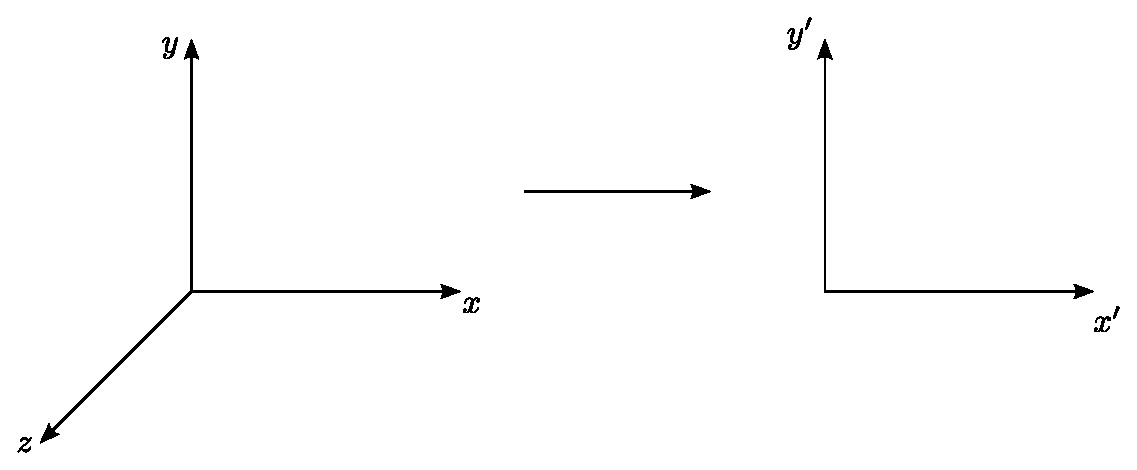
\includegraphics[width=0.4\linewidth,height=0.15\linewidth]{images/Trans.pdf}
\end{figure}To get the point $p'=\begin{pmatrix}
x' \\ y' \\ 0\\1
\end{pmatrix}$ from the point $p=\begin{pmatrix}
x \\ y \\ z\\1
\end{pmatrix}$ we must divide z in half and project it on the x/y-axis and must add this to the x/y value.
Projection:
\begin{figure}[!h]
	\centering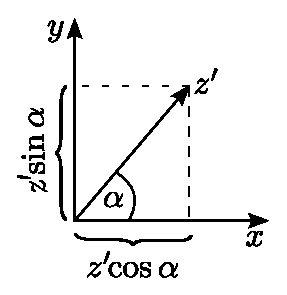
\includegraphics[width=0.3\linewidth,height=0.3\linewidth]{images/projection.pdf}
\end{figure}
\\The z' in the picture equals -0.5z $\Rightarrow p'=\begin{pmatrix}
x-0.5cos(\alpha)z\\
y-0.5cos(\alpha)z\\
0\\
1
\end{pmatrix}
$
\\$p'=M p\Longleftrightarrow \begin{pmatrix}
x-0.5cos(\alpha)z\\
y-0.5cos(\alpha)z\\
0\\
1
\end{pmatrix}= \begin{pmatrix}
a & b& c& d\\
e& f& g& h\\
i& j & k& l\\
m & n& o& q
\end{pmatrix}
\begin{pmatrix}
x\\
y\\
z\\
1
\end{pmatrix}=\begin{pmatrix}
ax+by+cz+d\\
ex+fy+gz+h\\
ix+jy+kz+l\\
mx+ny+oz+q
\end{pmatrix}
$
\\$\Rightarrow M= \begin{pmatrix}
1 & 0& -0.5 \cos(\alpha)& 0\\
0& 1& -0.5 \cos(\alpha)& 0\\
0& 0 & 0& 0\\
0 & 0& 0& 1
\end{pmatrix}$
\\ With $\alpha=45^\circ$ and $\cos(45^\circ)=\sin(45^\circ)=\frac{1}{\sqrt{2}}$ we get:
 $M= \begin{pmatrix}
1 & 0& -\frac{1}{2\sqrt{2}}& 0\\
0& 1& -\frac{1}{2\sqrt{2}}& 0\\
0& 0 & 0& 0\\
0 & 0& 0& 1
\end{pmatrix}$

\exercise{4.3}{ Perspective projection and lines } 
We want to understand the effects of perspective projection on lines in three dimensional
space.
Let $f>0$ be some constant. 
We omit the discussion of all the tricks with the third component of the projection (
which are relevant only for the z-buffer),
and we also omit all the details related to hardware-specific screen sizes and sign-conventions.
Instead, we assume without loss of generality, that the observer is located at $0$ and
is looking into the positive $z$-direction, projecting everything on a near-clipping
plane at $z=f$. That means, that a point $(x,y,z)$ is projected to $(fx/z, fy/z, f)$.
Expressed as a matrix for homogeneous coordinates, this looks as follows:
\[
  \mat{cccc}{
     f & 0 & 0 & 0 \\
     0 & f & 0 & 0 \\
     0 & 0 & f & 0 \\
     0 & 0 & 1 & 0 
  }
  \mat{c}{
    x \\
    y \\
    z \\
    1
  }
  = 
  \mat{c}{
    fx \\
    fy \\
    fz \\
    z 
  } 
  \rightharpoonup 
  \mat{c}{
    fx/z \\ 
    fy / z \\
    f
  }
\]
Now let $b\in \Real^3$ be some base vector and $d\in \Real^3$ be some dimension vector, we 
want to consider the straight line $\setPredicate{b + t d}{t\in\Real}$.
Applying the projection to the points of the straight line, we obtain:
\[
  \mat{cccc}{
     f & 0 & 0 & 0 \\
     0 & f & 0 & 0 \\
     0 & 0 & f & 0 \\
     0 & 0 & 1 & 0 
  }
  \mat{c} {
    b_x + t d_x \\
    b_y + t d_y \\
    b_z + t d_z \\
    1
  }
  \rightharpoonup
  \mat{c}{
    f \frac{b_x + t d_x}{b_z + t d_z} \\
    f \frac{b_y + t d_y}{b_z + t d_z} \\
    f
  }
\]
Now we want to compute the derivative of the right-hand side with respect to $t$.
Obviously, it is sufficient to consider only the first component (the 
second looks almost the same, the third is a constant). Let's also drop the
factor $f$ for a moment. It holds:
\begin{align*}
  \frac{d}{dt} \frac{b_x + t d_x}{b_z + t d_z} 
    &= \frac{d_x}{b_z + t d_z} - \frac{(b_x + t d_x) d_z}{(b_z + t d_z)^2} \\
    &= \frac{d_x(b_z + t d_z) - (b_x + t d_x) d_z}{(b_z + t d_z)^2} \\
    &= \frac{d_x b_z - b_x d_z}{(b_z + t d_z)^2}
\end{align*}
For all three components together, it means:
\begin{align*}
  \frac{d}{dt}\mat{c}{
    f \frac{b_x + t d_x}{b_z + t d_z} \\
    f \frac{b_y + t d_y}{b_z + t d_z} \\
    f
  } = 
  \frac{f}{(b_z + t d_z)^2}
  \mat{c}{
     d_x b_z - b_x d_z \\
     d_y b_z - b_y d_z \\
     0
  }.
\end{align*}
Now we can make the following observations.
First, notice that although the whole velocity vector is not constant, 
\emph{it's direction is}: it is always the vector $(
     d_x b_z - b_x d_z,
     d_y b_z - b_y d_z, 0
  )$, scaled by some $t$-dependent factor. 
  In particular, the projection of the line is contained in the 
  line 
  $\setPredicate{(f b_x / b_z, f b_y / b_z, f) + q (d_x b_z - b_x d_z,
  d_y b_z - b_y d_z, 0)}{q \in \Real}$. 
  If one does not care too much 
  about the fact that the original line is infinite, while the projected 
  line is bounded by vanishing points, one could express it as ``
  straight lines are projected to straight lines'' (this is the statement (i)).
  
  Now take a closer look at the direction vector $(d_x b_z - b_x d_z,
  d_y b_z - b_y d_z, 0)$. As long as $d_z$ is not zero, this direction 
  vector depends on the coordinates of the base point $b_x$ and $b_y$,
  so that parallel lines with $d_z\neq 0$ will in general no
  longer be parallel after projection (this shows (ii)).

  However, if $d_z$ is zero, then
  the direction vector becomes just $b_z(d_x, d_y, 0)$ after projection, that is, it is a scaled version of the original vector $(d_x, d_y, d_z)$. This means that
  parallel lines that are parallel to the projection plane remain parallel, 
  and do not intersect in a vanishing point (iii).
\end{document}
